\section{Baseline Design Validation and Projected Photon Detector Performance}
\label{sec:dp-pds-performance}

Since our initial simulation studies described in the \dshort{tp} \cite{Abi:2018rgm}, much progress has been made to advance towards a more realistic understanding of the projected \dshort{pds} performance using the \dshort{larsoft} framework:
%
\begin{itemize}
\item Optical simulations are now performed in the \dword{dp} \dword{fd} module geometry. In the \dword{fd} \dshort{tp}, physics studies assumed the \dword{pddp} geometry. Considering the lack of any optical segmentation in the \dword{dp} design, light is simulated in the full \dpactivelarmass \dshort{tpc} active volume. The simulations assume a \SI{61}{\cm} Rayleigh scattering length in \lar, a \SI{20}{\m} absorption length in \lar and fully absorptive field cage surfaces, for \SI{127}{\nm} light. For each one of the \dpnumpmtch \dwords{pmt}, simulations take into account how the photon detection probabilities and the photon propagation times vary throughout the \dshort{tpc} active volume.
%
\item The simulation of the electronics response, as well as the reconstruction of optical hits and optical clusters, is now accounted for. The electronics simulation includes \dshort{pmt} dark counts at \SI{1.7}{\kHz} rate, waveform digitization at \SI{250}{\MHz} sampling rate, \dshort{pmt} gain at \num{e7} (corresponding to about \SI{25}{ADC counts per PE}) and electronics noise of \SI{0.8}{ADC counts RMS}. The assumed single-PE to baseline noise RMS ratio is therefore about \num{30}. Optical hits are the reconstructed optical signals on single \dshort{pmt} waveforms, and are characterized by a hit time, amplitude, and charge. Optical clusters refer to a collection of \dshort{pmt} hits that are correlated in time and space. They are typically induced by the same underlying flash of scintillation light in \lar. The parameters of the clustering algorithm are discussed later in this section.

\fixme{Need to repeat the studies for a \SI{15.4}{\ns} sampling and a correspondingly reduced S/N ratio (latter number TBD, check with Antonio).}

%
\item The physics studies now also include radiological backgrounds. The simulation of radiological backgrounds is critical in order to perform a realistic optimization of the optical reconstruction parameters. The radiological model includes several radio-isotopes throughout the \lar volume, with \SI{1.01}{\becquerel/\kg} of $^{39}$Ar providing the largest activity. In addition, an impinging neutron flux of \SI{e-5}{\cm$^{-2}$\s$^{-1}$} is accounted for.
\end{itemize} 

\fixme{Need to check that neutron component of radiological model is implemented correctly}

Figure~\ref{fig:dppd_light_yield} shows the expected incident light yield, in units of number of photons reaching the \dword{pmt} windows per MeV of deposited energy, and for energy depositions throughout the \dword{dp} \dshort{fd} cryostat. In order to obtain the detected light yield, in PEs/MeV units, the numbers should be multiplied by an effective quantum efficiency of 0.12. In the left panel, the incident light yield is shown as a function of the X (vertical and parallel to drift) and Y (horizontal and perpendicular to neutrino beam) coordinates, while averaging over the Z coordinate enclosed in the \dword{tpc} active volume (not shown). The red contour indicates the \dshort{tpc} active volume. The right panel shows the trend as a function of X only, averaging over Y and Z simultaneously. In this way, one appreciates better the main trend in the spatial response, namely the light yield reduction with increasing distance from the cathode. The incident light yield is expected to be as high as \num{2e2} photons/\si{\MeV} near the cathode surface, and of order \num{0.5} photons/\si{\MeV} near the liquid-gas interface. 

\begin{dunefigure}[Expected light yield in the full \dword{dp} \dshort{fd} cryostat.]{fig:dppd_light_yield}
     {Expected incident light yield in the full \dword{dp} \dshort{fd} cryostat. The yield units are the number of photons reaching the PMT windows per \si{\MeV} of deposited energy. Left panel: yield as a function of the X (vertical and parallel to drift) and Y (horizontal and perpendicular to neutrino beam) coordinates, averaging over the Z coordinate (not shown). The red contour indicates the \dshort{tpc} active volume. Right panel: yield as a function of X, averaging over Y and Z. The \dwords{pmt} are located at X=\SI{-7}{\m}.}
    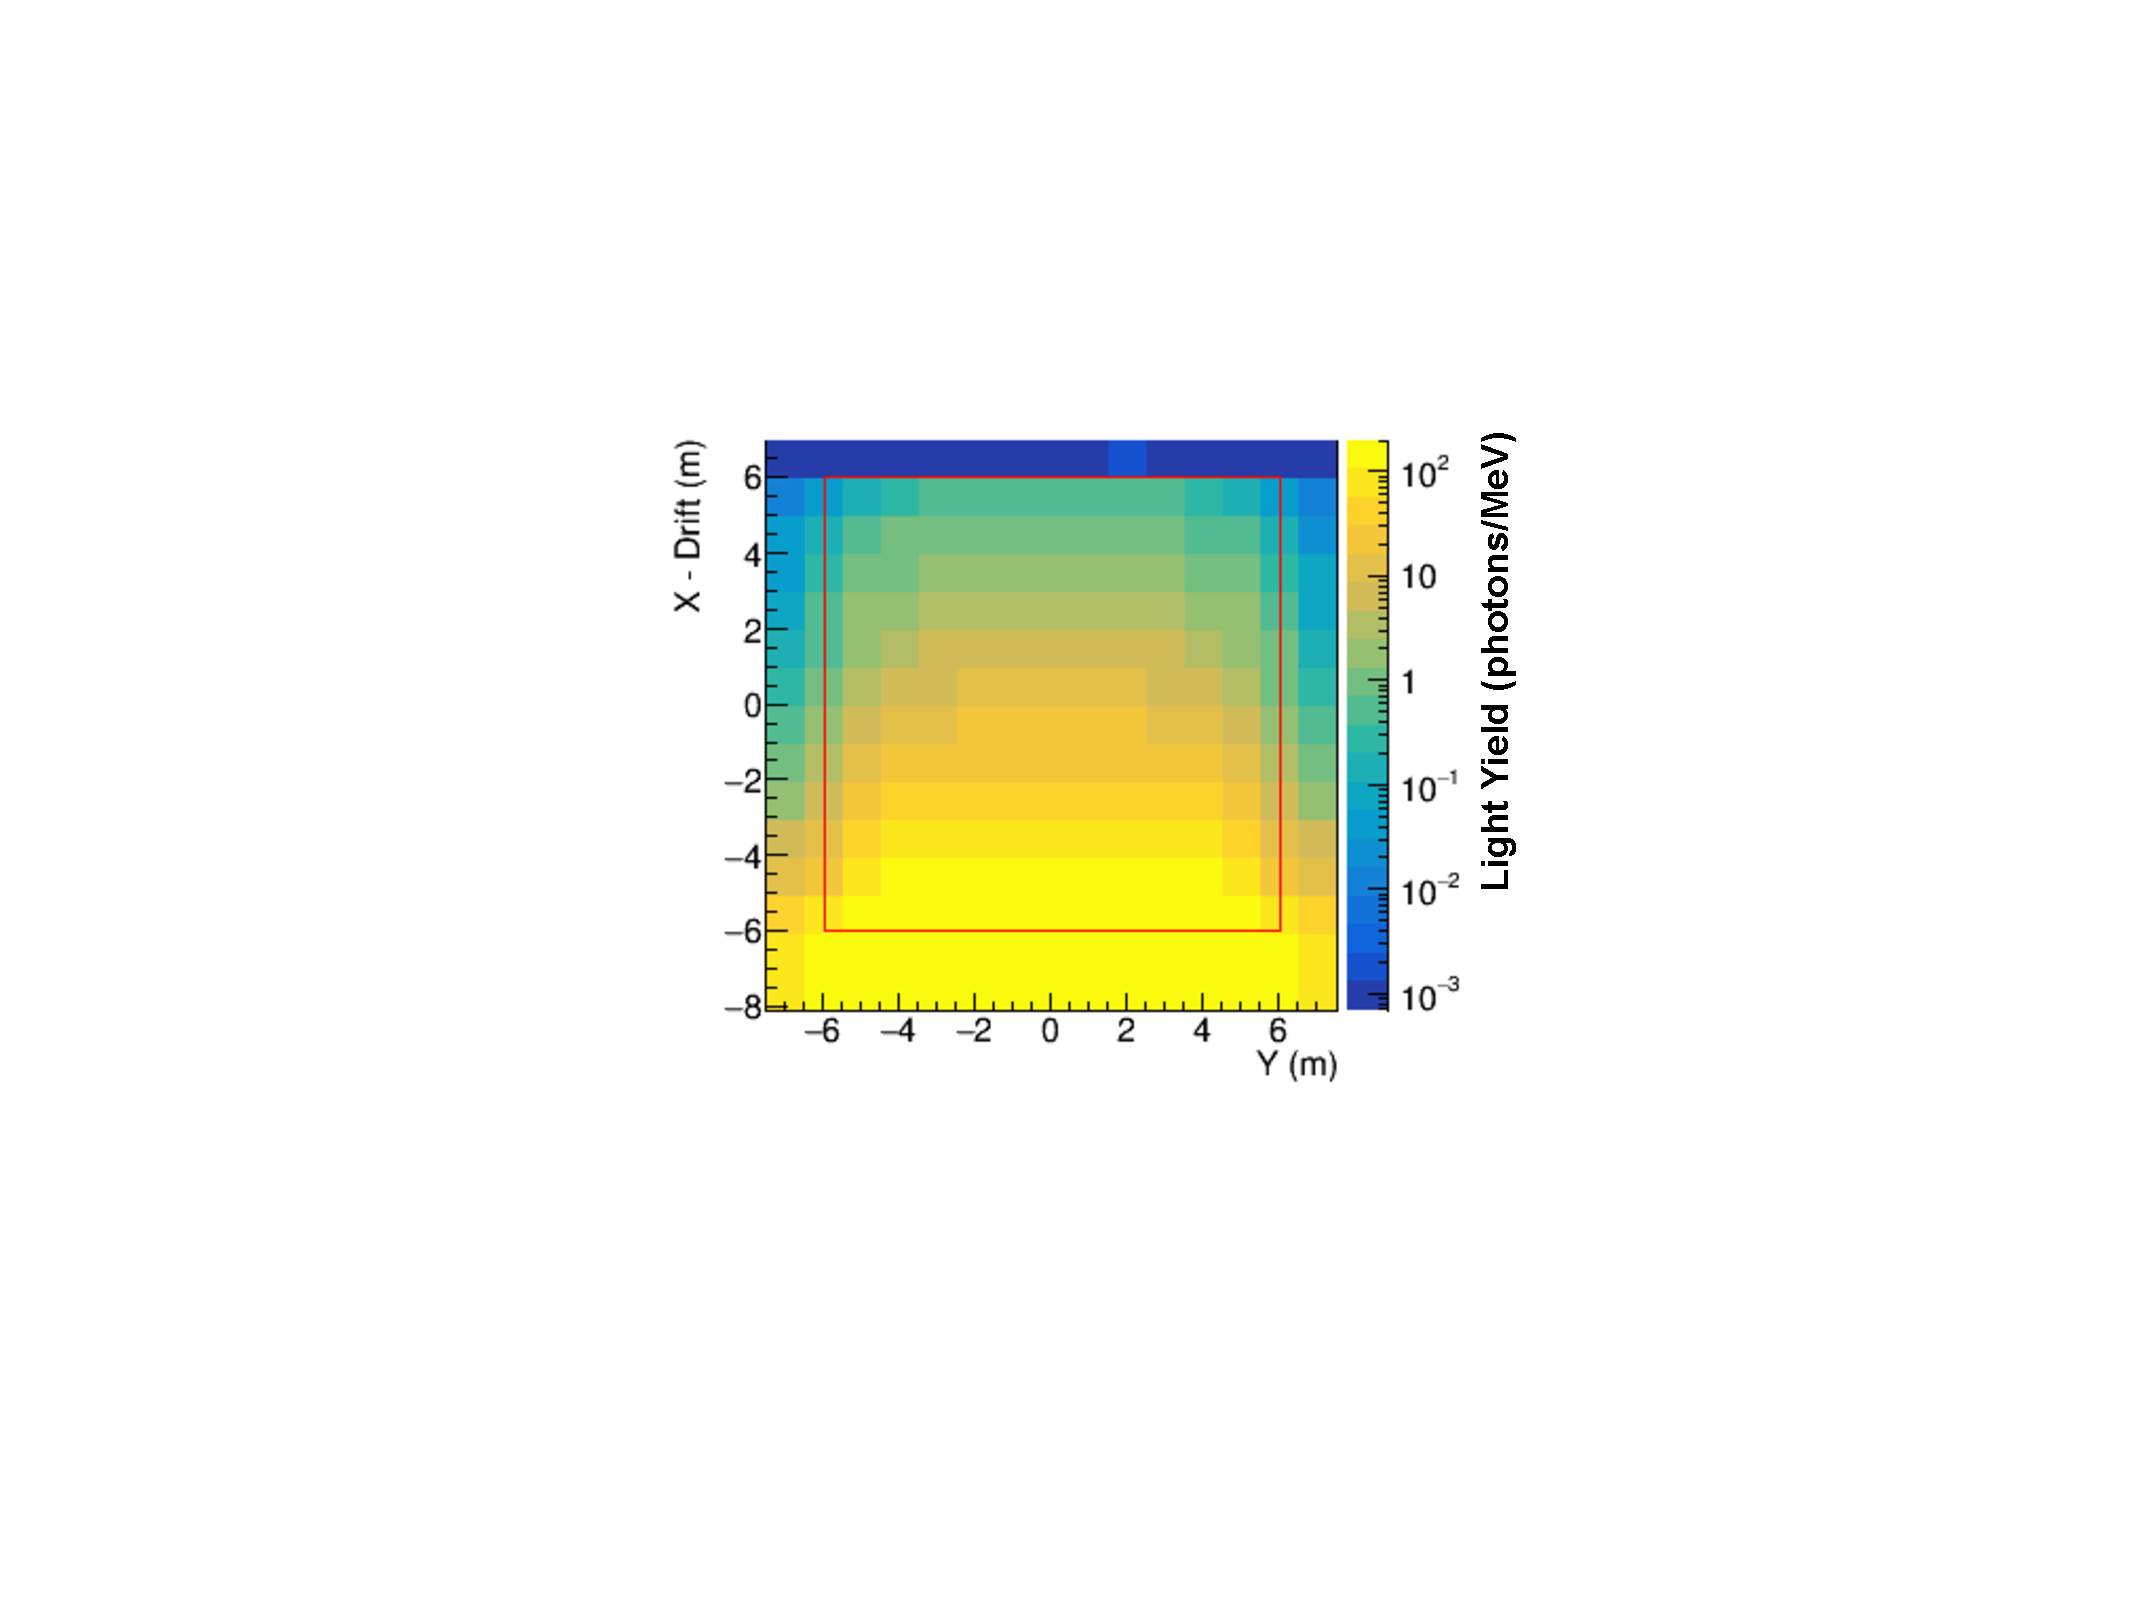
\includegraphics[width=0.49\textwidth]{graphics/dppd_light_yield_2D.pdf} \hfill
    \raisebox{0.5cm}{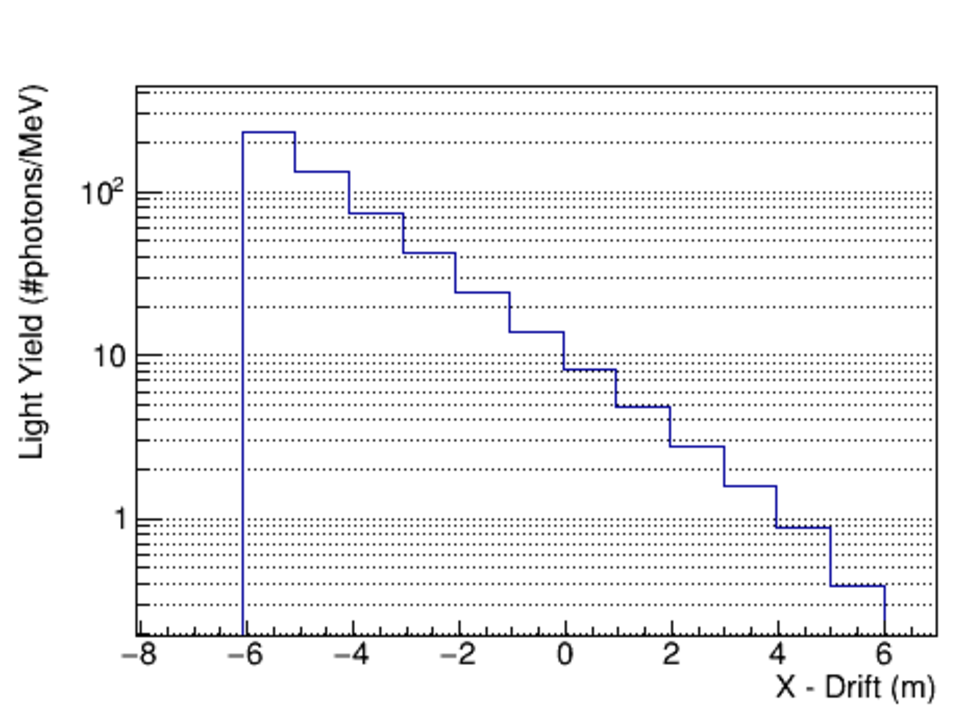
\includegraphics[width=0.49\textwidth]{graphics/dppd_light_yield_1D.pdf}}
    \end{dunefigure}

\fixme{Produce light maps and all plots in this section also for the case of \dword{wls} reflector foils on the field cage. This is the highest priority item in this section.}

%%%%%%%%%%%%%%%%%%%%%%%%%%%%%%%%%%%%%%%%%%%%%%%%%%%%%%%%%%%%%%%%%%%%

\subsection{Event $t_{0}$ Reconstruction}

As discussed in Sec.~\ref{sec:dp-pds-requirements}, event $t_0$ reconstruction for non-beam events via the \dshort{pds} is particularly important in order to be able to fiducialize nucleon decay candidates in \dword{dune}. Proton decay signal events with a \ptoknubar final state have been simulated with GENIE \cite{Andreopoulos:2009rq} throughout the \dword{dp} \dshort{tpc} active volume, and their optical clusters were reconstructed according to the simulation and reconstruction chain described above. NDK events are expected to deposit about \SI{400}{\MeV} visible energy in the \lar. The same reconstruction algorithm has also been applied to the simulated radiological backgrounds. Four optical cluster reconstruction parameters have been optimized:
\begin{description}
\item[Maximum cluster duration:] maximum time difference between all \dshort{pmt} hits in the cluster. The optimal value was found to be \SI{1}{\us}.
\item[Maximum hit time distance:] maximum time difference between successive \dshort{pmt} hits in the cluster. By definition, this quantity should be smaller than the maximum cluster duration. The optimal value was found to be \SI{800}{\ns}.
\item[Maximum hit distance:] maximum spatial distance between neighbouring \dshort{pmt} hits in the cluster. The optimal value was found to be \SI{2.5}{\m}. Recalling that the \dwords{pmt} are located on a square lattice with \SI{1}{\m} pitch, a \SI{2.5}{\m} maximum hit distance means that the cluster can contain gaps in its hit pattern along a single \dshort{pmt} row or column.
\item[Minimum cluster charge:] minimum number of reconstructed PEs per cluster. This parameter is particularly important, since the radiological background cluster rate is very sensitive to it. The optimal value for the charge threshold was found to be \num{87} PEs, for an average background  rate of \num{0.1} clusters per \dpreadout readout window. The latter number was set to ensure a \SI{>90}{\%} purity in associating the correct optical flash to the NDK energy deposition, as discussed in Sec.~\ref{subsec:dp-pds-requirements_requirements}.
\end{description} 

Figure~\ref{fig:dppd_ndk_optimization} illustrates the optimization process of the cluster parameters for NDK $t_{0}$ reconstruction and justifies the choice of some of those parameters. For each chosen set of (maximum cluster duration, maximum hit time distance, maximum hit distance) parameters, the minimum cluster charge is set to a value that yields a tolerable radiological background rate. As discussed in Sec.~\ref{sec:dp-pds-requirements}, we require a $>90\%$ NDK flash purity among all reconstructed NDK-like flashes within the same NDK event readout window to minimise $t_0$ reconstruction ambiguities. For this reason, we set the tolerable radiological background rate to 0.1 clusters per readout window, on average. Once the minimum cluster charge parameter is set in this way, the combination of the four cluster parameters determines the NDK signal efficiency. We repeat this process by scanning various choices of the (maximum cluster duration, maximum hit time distance, maximum hit distance) parameters, setting the minimum cluster charge to values meeting the tolerable background rate in each case. Figure~\ref{fig:dppd_ndk_optimization} shows that, for a \SI{1}{\micro\s} maximum cluster duration, indeed the maximum hit time distance and maximum hit distance parameters that maximize the NDK signal efficiency are \SI{800}{\ns} and \SI{2.5}{\m}, respectively, as stated above. For these parameters, the minimum cluster charge is set to \SI{87}{PEs} and the NDK $t_0$ reconstruction efficiency averaged over the entire \dshort{tpc} active volume is \SI{55.5}{\%}.

\begin{dunefigure}[Optimization of optical cluster parameters for NDK events.]{fig:dppd_ndk_optimization}
     {Optimization of optical cluster parameters for NDK events. For a \SI{1}{\us} maximum cluster duration, the maximal NDK signal efficiency of \num{55.5}\% is achieved for an \SI{800}{\ns} maximum hit time distance and a \SI{2.5}{\m} maximum hit distance. The 2D histogram colors indicate the $t_0$ reconstruction efficiency, and the charge (in PEs) within each box shows the minimum cluster charge that yields \num{0.1} average background cluster rate per readout window. See text for details.}
    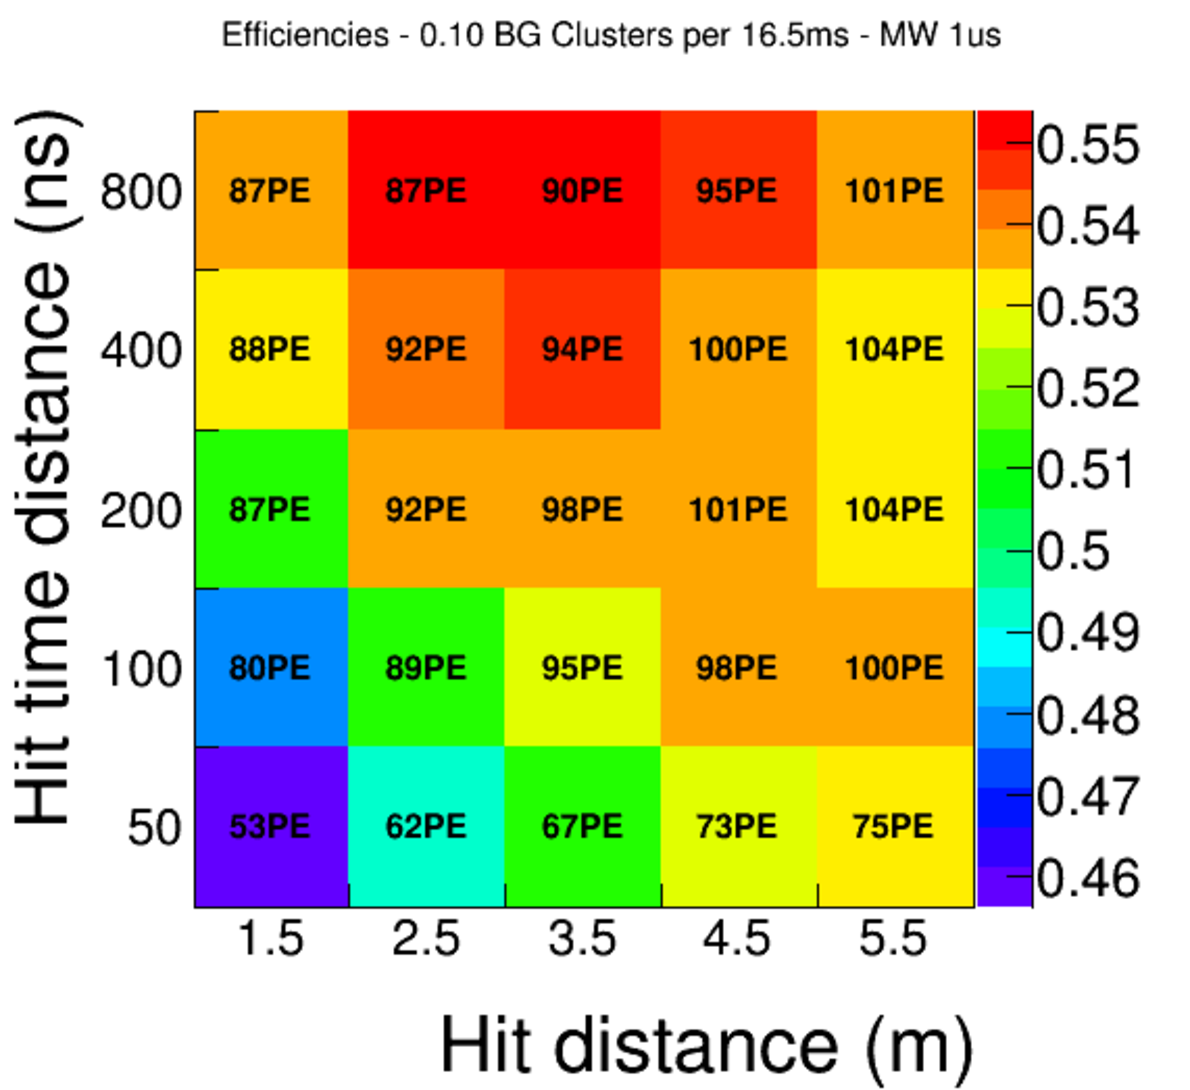
\includegraphics[width=0.5\textwidth]{graphics/dppd_ndk_optimization.pdf}
    \end{dunefigure}

Figure~\ref{fig:dppd_ndk_efficiencies} shows how the NDK $t_0$ reconstruction efficiency varies as a function of the nucleon decay vertex distance from the cathode plane, and for different choices of tolerable background cluster rates. Our nominal curve is the red one, corresponding to \num{0.1} background clusters on average. As can be seen, the efficiency remains $>90\%$ for distances up to \SI{6}{\m} from the cathode. However, the efficiency drops rapidly for distances beyond that, resulting in the \num{55.5}\% average efficiency quoted above. This efficiency drop is caused by the marked reduction in the detected light yield as the energy deposition occurs at increasingly larger distances from the cathode, see Fig.~\ref{fig:dppd_light_yield}. Figure~\ref{fig:dppd_ndk_efficiencies} also shows how the NDK $t_0$ reconstruction efficiency varies with different choices of the tolerable background cluster rate. Obviously, the higher the tolerable background rate, the higher the NDK signal efficiency. However, the marked efficiency drop for increasing nucleon decay vertex distance from the cathode remains for all choices.

\begin{dunefigure}[Nucleon decay $t_0$ reconstruction efficiency.]{fig:dppd_ndk_efficiencies}
     {Nucleon decay $t_0$ reconstruction efficiency as a function of decay vertex distance from the cathode, and for two different choices of tolerable radiological background cluster rates per readout window.}
    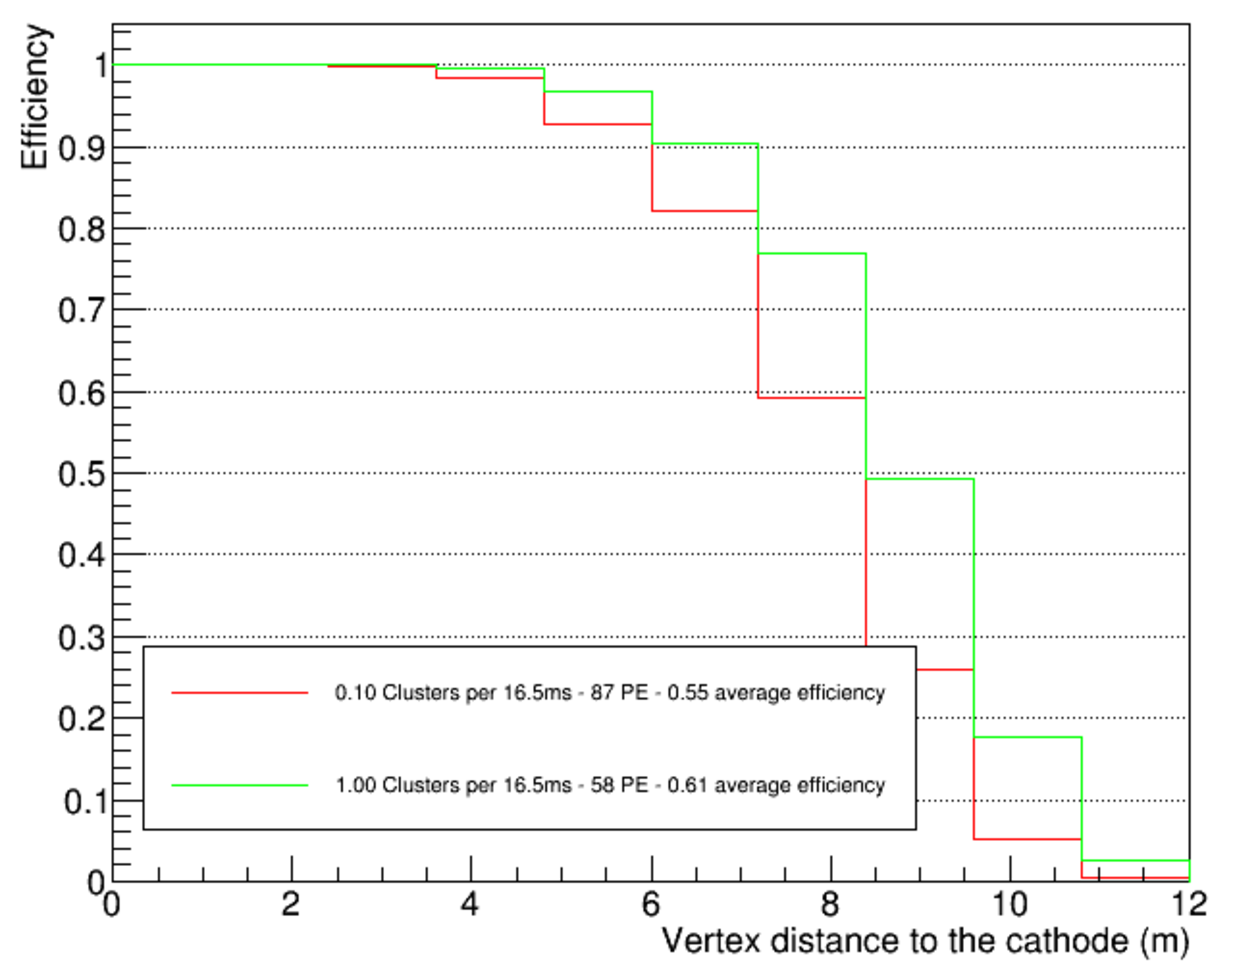
\includegraphics[width=0.5\textwidth]{graphics/dppd_ndk_efficiencies.pdf}
    \end{dunefigure}


\fixme{Update NDK plots to include two cases: with and without foils.}

\fixme{Update NDK plots to include improvements to clustering algorithm, e.g. use of cluster reconstructed spatial location to reduce mis-associations with radiological clusters.}

A similar study has been performed also on SN \nue \dword{cc} interactions generated with Marley \cite{marley}. Compared to the NDK case, the reconstructed optical signals are much weaker, since the typical deposited energies per SN neutrino interaction are of order \SI{20}{\MeV}. For a much lower radiological background rate of \SI{0.5}{\Hz}, about ten times lower than what was assumed in the NDK case, an average SN $t_0$ reconstruction efficiency of \SI{15.0}{\%} is obtained from our studies. This value of radiological background rate was found by optimizing the SN burst triggering efficiency, see below. 

%%%%%%%%%%%%%%%%%%%%%%%%%%%%%%%%%%%%%%%%%%%%%%%%%%%%%%%%%%%%%%%%%%%%

\subsection{Supernova Burst Triggering}

We have also studied the capability of the \dword{dp} \dshort{pds} to trigger on a SN burst occurring in our galactic neighbourhood. As described in Sec.~\ref{sec:dp-pds-requirements}, this is one of the primary goals of the system. In \dword{dune}, a real-time algorithm is expected to provide trigger primitives by searching for \dshort{pmt} hits and optical clusters, where the latter combine several hits together based on their time/spatial information. The process is therefore similar to the offline cluster reconstruction discussed above. 

The computation of the \dshort{pds}-based trigger efficiency for SN bursts as a function of SN distance has been computed as follows:

\begin{itemize}
\item In a first step, the minimum number of reconstructed clusters required in a \SI{5}{\s} time window in order to issue a trigger is found\footnote{A \SI{5}{\s} time window was found to be nearly optimal and is assumed throughout this section.}. The minimum cluster multiplicity is set by the requirement of one fake trigger per month at most (see Sec.~\ref{sec:dp-pds-requirements}), and by the radiological background cluster rate. The higher the background cluster rate, the higher the minimum cluster multiplicity has to be in order to meet the $<$\num{1}/month fake trigger rate requirement. As mentioned above, a clustering optimization procedure similar to the one described for NDK events yields a background cluster rate of \SI{0.5}{\Hz}, or \num{2.5} clusters per \SI{5}{\s} window, on average. For such a background rate level, a minimum cluster multiplicity of $>$\num{13} per \SI{5}{\s} time window is required for a $<$\num{1}/month fake trigger rate.
%
\item In a second step, and given the cluster parameters and the minimum cluster multiplicity defined in the first step, the SN burst triggering efficiency as a function of the number of SNB interactions is computed. For a \SI{15.0}{\%} average efficiency of reconstructing single SN \nue interactions with the \dshort{pds} and a minimum cluster multiplicity of \num{13} in order to issue a trigger, about \num{13}/\num{0.15}$\simeq$ \num{90} interactions have to occur in the FD module and within \SI{5}{\s} in order to obtain a non-negligible trigger efficiency. 
%
\item In a third and final step, the SN burst triggering efficiency as a function of SN distance is obtained. We use the theoretical assumptions shown in Fig.~\ref{fig:dppd_snbassumptions} to extract the number of SN neutrino interactions in a \SI{5}{\s} time window and in one \dword{dp} \dword{fd} module as a function of SN distance. The left panel of Fig.~\ref{fig:dppd_snbassumptions} shows the time-integrated expected number of SN neutrino interactions as a function of distance, while the right panel in Fig.~\ref{fig:dppd_snbassumptions} shows the assumed time profile of the burst during the first \SI{10}{\s}. Several hundred SN neutrino interactions are expected in one DP FD module for a \SI{10}{\kilo\parsec} distant SN, and the vast majority of them are expected within the first \SI{5}{\s}. Given our earlier estimate that about \num{90} interactions are expected to be sufficient for a non-negligible trigger efficiency, it is clear that the \dshort{pds} should provide a high SN burst trigger efficiency for a SN at a \SI{10}{\kilo\parsec} distance.
\end{itemize}

\begin{dunefigure}[SN burst triggering assumptions.]{fig:dppd_snbassumptions}
     {Left panel: expected number of SN \nue \dshort{cc} interactions in one \dpactivelarmass active mass DP module as a function of SN distance. The different red lines indicate different SN burst models. Right panel: expected time profile of the SN burst.}
    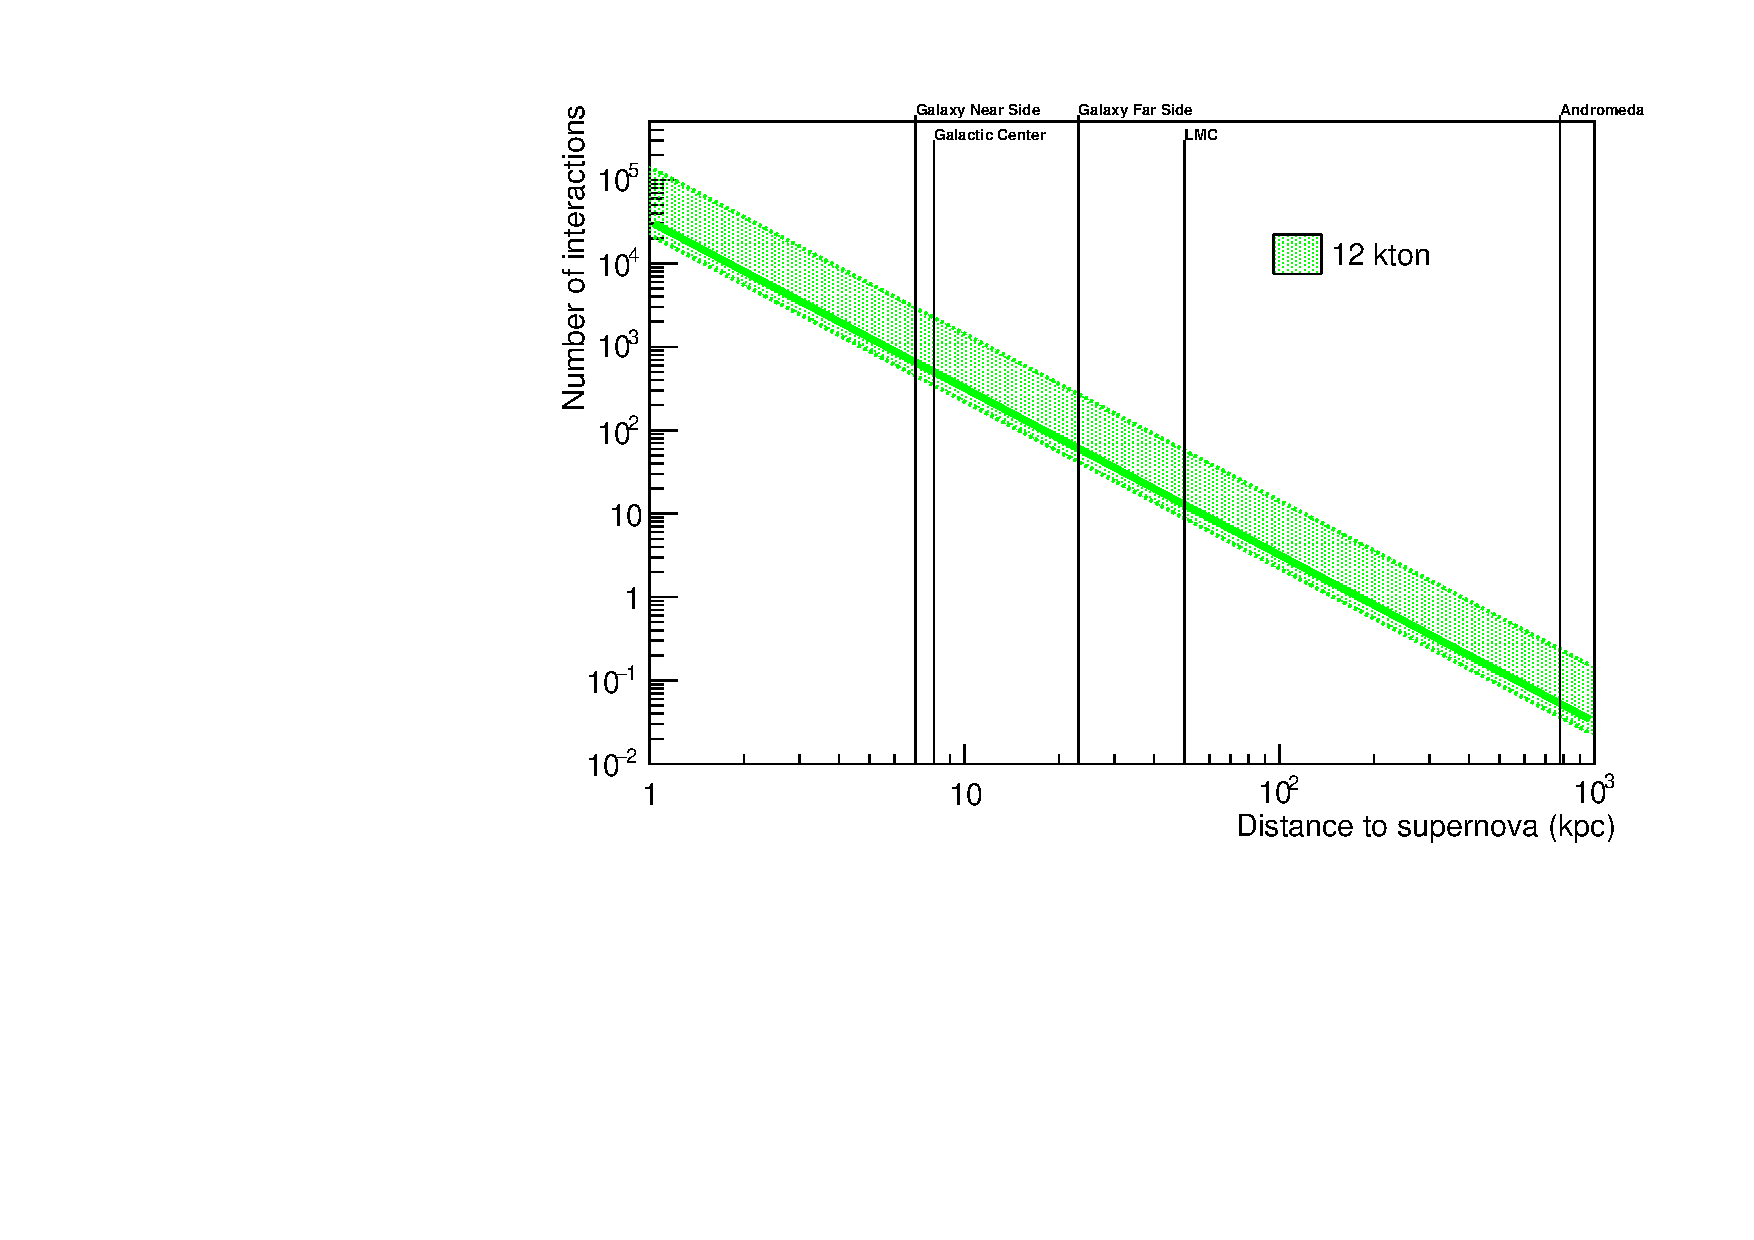
\includegraphics[width=0.49\textwidth]{graphics/dppd_events_vs_sndistance.pdf} \hfill
    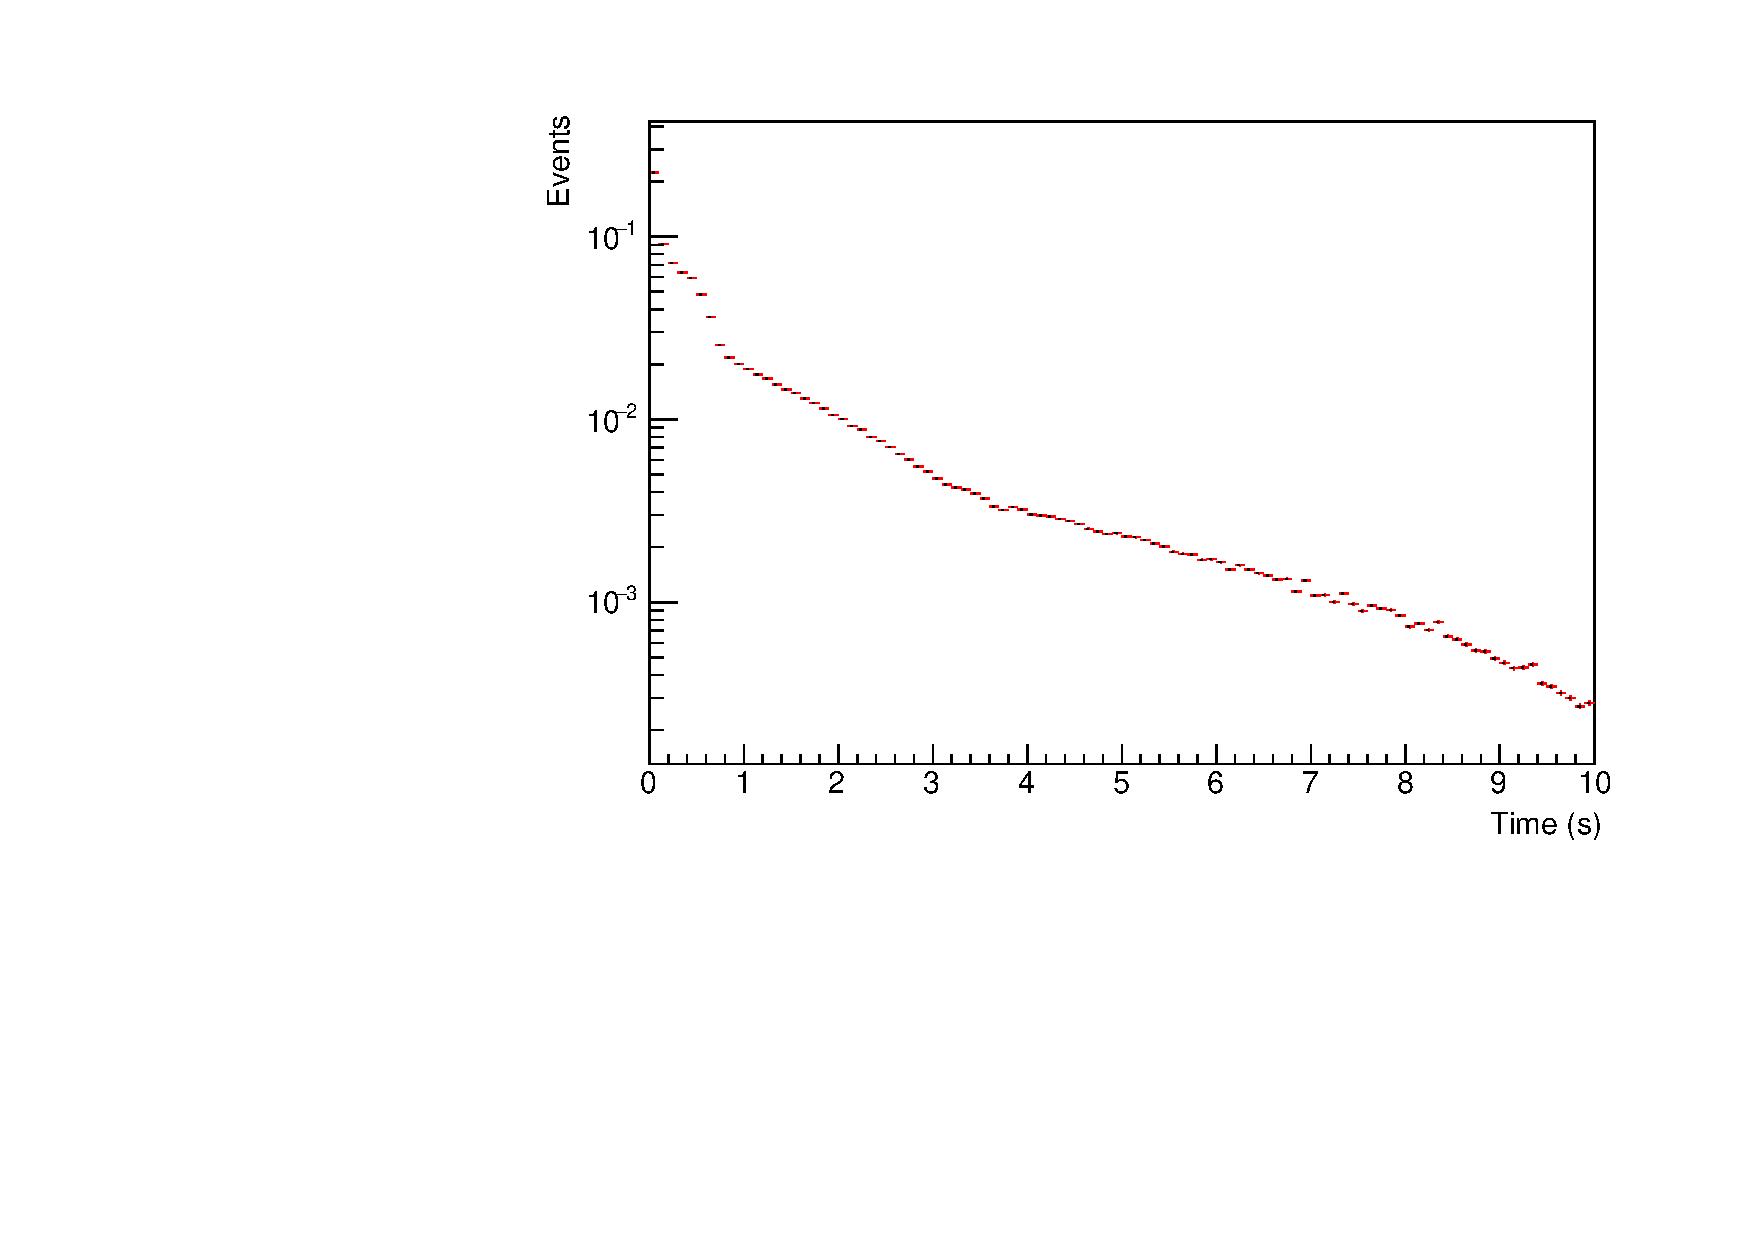
\includegraphics[width=0.49\textwidth]{graphics/dppd_sntime_profile.pdf} 
    \end{dunefigure}

The SN burst triggering efficiency, computed following the procedure described above and as a function of SN distance, is shown in Fig.~\ref{fig:dppd_snbefficiency_vs_sndistance}. The figure shows how the SN burst triggering efficiency is affected by different choices of the cluster reconstruction parameters. The best trigger efficiency is found for the cluster parameters yielding the lowest background cluster rates, in the \SIrange{0.25}{0.5}{\Hz} range. In this case, a trigger efficiency in excess of \num{90}\% is obtained up to SN distances of about \SI{18}{\kilo\parsec}. Therefore, the \dshort{pds} is expected to yield a highly efficient trigger for SN bursts occurring anywhere in the Milky Way.

\begin{dunefigure}[SN burst triggering efficiency.]{fig:dppd_snbefficiency_vs_sndistance}
     {SN burst triggering efficiency using \dword{dp} \dshort{pds} information as a function of SN distance. Different curves indicate different choices of the optical cluster reconstruction parameters.}
    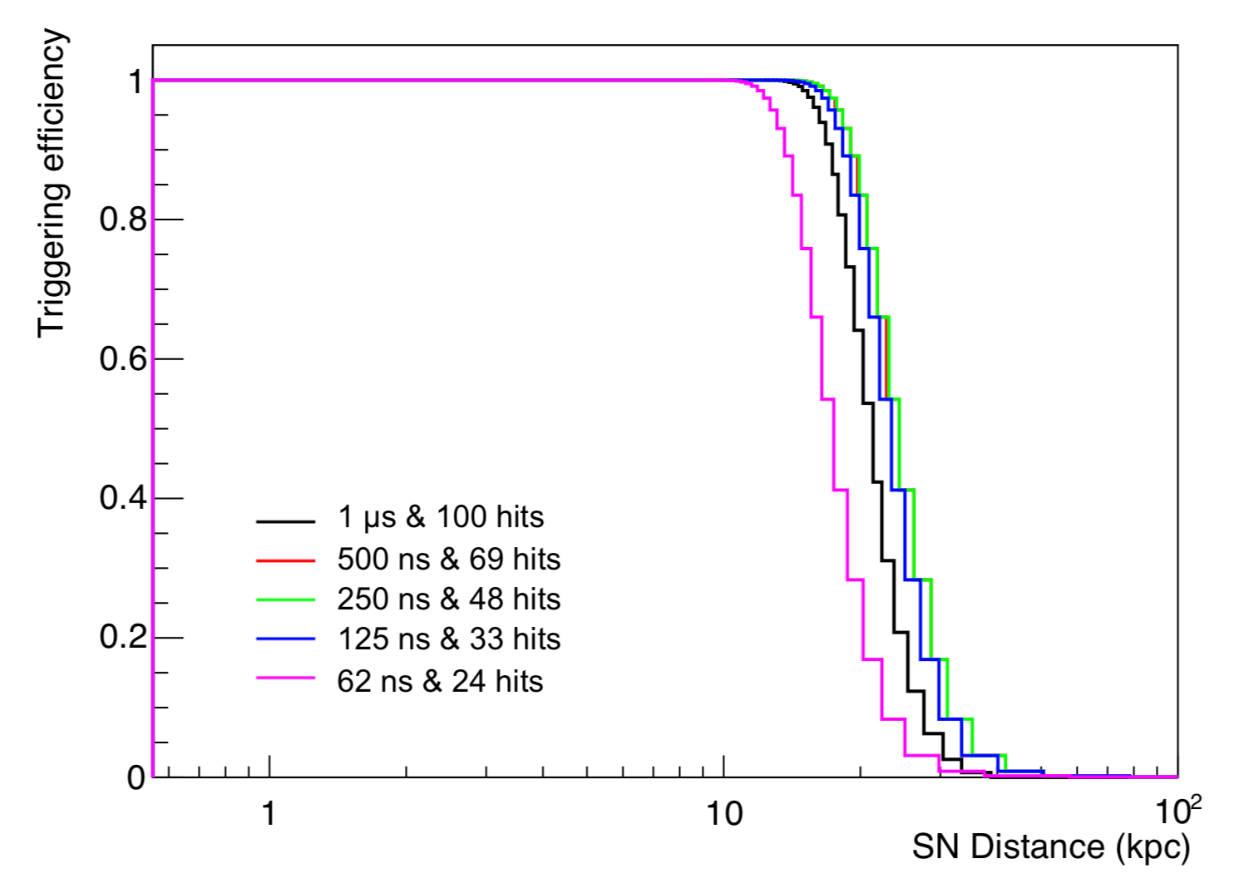
\includegraphics[width=0.6\textwidth]{graphics/dppd_snbefficiency_vs_sndistance.pdf}
    \end{dunefigure}

\fixme{Update SNB plots to include two cases: with/without reflector foils.}

\fixme{Update SNB plots with x10 increase in radiological MC statistics.}

\fixme{Update SNB plots with updated clustering algorithm.}

\fixme{Update SNB plots with optimized time window (\SI{2.5}{\s})?}


%%%%%%%%%%%%%%%%%%%%%%%%%%%%%%%%%%%%%%%%%%%%%%%%%%%%%%%%%%%%%%%%%%%%

\subsection{Event Energy Reconstruction}

\fixme{Add study with simulated beam \nue \dword{cc} interactions to justify choice of \SI{200}{PEs} dynamic range in Tab.~\ref{tab:specs:just:DP-PDS}, or change number accordingly. Study to be done for two samplings: \SI{15.4}{\ns} and \SI{400}{\ns}.}

\fixme{Add full study of PDS-based energy reconstruction performance, using simulated beam \nue \dword{cc} interactions.} 